\documentclass{standalone}
\usepackage{tikz}
\usepackage{ctex,siunitx}
\setCJKmainfont{Noto Serif CJK SC}
\usepackage{tkz-euclide}
\usepackage{amsmath}
\usetikzlibrary{patterns, calc}
\usetikzlibrary {decorations.pathmorphing, decorations.pathreplacing, decorations.shapes,}
\begin{document}
\small
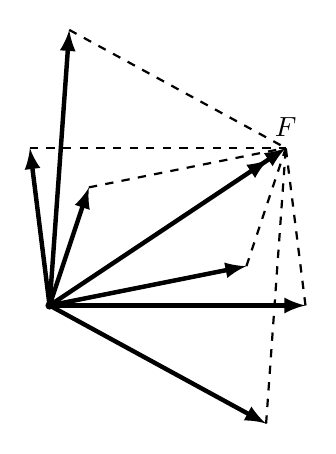
\begin{tikzpicture}[>=latex, thick,scale=1]
  % \useasboundingbox(-1,-0.75)rectangle(3.7,1.4);
  \fill (0,0) circle[radius=1.5pt];
  \draw [->>, ultra thick](0,0)--(3,2) node [above] {$F$};
  \draw [->, ultra thick](0,0)--(.5,1.5) ;
  \draw [dashed](.5,1.5)--(3,2) ;
  \draw [->, ultra thick](0,0)--(2.5,.5) ;
  \draw [dashed](2.5,.5)--(3,2) ;
  \draw [->, ultra thick](0,0)--(.25,3.5) ;
  \draw [dashed](.25,3.5)--(3,2) ;
  \draw [->, ultra thick](0,0)--(2.75,-1.5) ;
  \draw [dashed](2.75,-1.5)--(3,2) ;
  \draw [->, ultra thick](0,0)--(-.25,2) ;
  \draw [dashed](-.25,2)--(3,2) ;
  \draw [->, ultra thick](0,0)--(3.25,0) ;
  \draw [dashed](3.25,0)--(3,2) ;
\end{tikzpicture}
\end{document}